\documentclass[10pt,landscape]{article}

\usepackage{multicol}
\usepackage{calc}
\usepackage{ifthen}
\usepackage[landscape]{geometry}
\usepackage{graphicx}
\usepackage{amsmath, amssymb, amsthm}
\usepackage{latexsym, marvosym}
\usepackage{pifont}
\usepackage{lscape}
\usepackage{graphicx}
\usepackage{array}
\usepackage{booktabs}
\usepackage[bottom]{footmisc}
\usepackage{tikz}
\usetikzlibrary{shapes}
\usepackage{pdfpages}
\usepackage{wrapfig}
\usepackage{enumitem}
\setlist[description]{leftmargin=0pt}
\usepackage{xfrac}
\usepackage[pdftex,
            pdfauthor={Janet Matsen},
            pdftitle={Machine Learning Cheatsheet},
            pdfsubject={Notes from UW CSE 446 Winter 2016},
            pdfkeywords={machine learning} {statistics} {cheatsheet} {pdf} {cheat} {sheet} {formulas} {equations}
            ]{hyperref}
\usepackage{relsize}
\usepackage{rotating}

 \newcommand\independent{\protect\mathpalette{\protect\independenT}{\perp}}
    \def\independenT#1#2{\mathrel{\setbox0\hbox{$#1#2$}%
    \copy0\kern-\wd0\mkern4mu\box0}} 
            
% Janet defined
\DeclareMathOperator*{\argmin}{arg\,min}
\DeclareMathOperator*{\argmax}{arg\,max}

% Probably from Stat cheatsheet:            
\newcommand{\noin}{\noindent}    
\newcommand{\logit}{\textrm{logit}} 
\newcommand{\var}{\textrm{Var}}
\newcommand{\cov}{\textrm{Cov}} 
\newcommand{\corr}{\textrm{Corr}} 
\newcommand{\N}{\mathcal{N}}
\newcommand{\Bern}{\textrm{Bern}}
\newcommand{\Bin}{\textrm{Bin}}
\newcommand{\Beta}{\textrm{Beta}}
\newcommand{\Gam}{\textrm{Gamma}}
\newcommand{\Expo}{\textrm{Expo}}
\newcommand{\Pois}{\textrm{Pois}}
\newcommand{\Unif}{\textrm{Unif}}
\newcommand{\Geom}{\textrm{Geom}}
\newcommand{\NBin}{\textrm{NBin}}
\newcommand{\Hypergeometric}{\textrm{HGeom}}
\newcommand{\HGeom}{\textrm{HGeom}}
\newcommand{\Mult}{\textrm{Mult}}

\geometry{top=.4in,left=.2in,right=.2in,bottom=.4in}

\pagestyle{empty}
\makeatletter
\renewcommand{\section}{\@startsection{section}{1}{0mm}%
                                {-1ex plus -.5ex minus -.2ex}%
                                {0.5ex plus .2ex}%x
                                {\normalfont\large\bfseries}}
\renewcommand{\subsection}{\@startsection{subsection}{2}{0mm}%
                                {-1explus -.5ex minus -.2ex}%
                                {0.5ex plus .2ex}%
                                {\normalfont\normalsize\bfseries}}
\renewcommand{\subsubsection}{\@startsection{subsubsection}{3}{0mm}%
                                {-1ex plus -.5ex minus -.2ex}%
                                {1ex plus .2ex}%
                                {\normalfont\small\bfseries}}
\makeatother

\setcounter{secnumdepth}{0}

\setlength{\parindent}{0pt}
\setlength{\parskip}{0pt plus 0.5ex}

% -----------------------------------------------------------------------

\usepackage{titlesec}

\titleformat{\section}
{\color{blue}\normalfont\large\bfseries}
{\color{blue}\thesection}{1em}{}
\titleformat{\subsection}
{\color{cyan}\normalfont\normalsize\bfseries}
{\color{cyan}\thesection}{1em}{}
% Comment out the above 5 lines for black and white

\begin{document}

\raggedright
\footnotesize
\begin{multicols*}{3}

% multicol parameters
% These lengths are set only within the two main columns
%\setlength{\columnseprule}{0.25pt}
\setlength{\premulticols}{1pt}
\setlength{\postmulticols}{1pt}
\setlength{\multicolsep}{1pt}
\setlength{\columnsep}{2pt}

%%%%%%%%%%%%%%%%%%%%%%%%%%%%%%%%%%%%
%%% TITLE
%%%%%%%%%%%%%%%%%%%%%%%%%%%%%%%%%%%%

\begin{center}
    {\color{blue} \Large{\textbf{Machine Learning Cheatsheet}}} \\
   % {\Large{\textbf{Probability Cheatsheet}}} \\
    % comment out line with \color{blue} and uncomment above line for b&w
\end{center}

%%%%%%%%%%%%%%%%%%%%%%%%%%%%%%%%%%%%
%%% ATTRIBUTIONS
%%%%%%%%%%%%%%%%%%%%%%%%%%%%%%%%%%%%

\scriptsize

Janet Matsen's Machine Learning (ML) notes from CSE 446, Winter 2016.  \url{http://courses.cs.washington.edu/courses/cse446/16wi/}

Used LaTeX template from an existing Statistics cheat sheet: \url{https://github.com/wzchen/probability_cheatsheet}, by William Chen (\url{http://wzchen.com}) and Joe Blitzstein. 

Licensed under \texttt{\href{http://creativecommons.org/licenses/by-nc-sa/4.0/}{CC BY-NC-SA 4.0}}. 

\begin{center}
    Last Updated \today
\end{center}

% Cheatsheet format from
% http://www.stdout.org/$\sim$winston/latex/

%%%%%%%%%%%%%%%%%%%%%%%%%%%%%%%%%%%%
%%% BEGIN CHEATSHEET
%%%%%%%%%%%%%%%%%%%%%%%%%%%%%%%%%%%%
  
    \hfill \\   
     \hfill \\  
\smallskip \hrule height 2pt \smallskip

\section{Essential ML ideas}
\smallskip \hrule height 2pt \smallskip

\begin{itemize}
	\item Never ever \underline{ever} touch the test set
	\item You know you are overfitting when there is a big test between train and test results.  E.g. metric of percent wrong. 
	\item Need to be comfortable taking a hit on fitting accuracy if you can get a benefit on the result.
	\item Bias vs variance trade-off.  
		High bias when the model is too simple \& doesn't fit the data well.  
		High variance is when small changes to the data set lead to large solution changes. 
	\item If features are non discriminative in the beginning, they don't work for any classifier.  % week 4 reminder
	\item Your feature vector often has a smaller dimension that the feature space.    % week 4, Friday. 
		If you have too long of a feature vector, you may get overfitting. 
	\item You need to prevent the optimizer from getting an easy way out.  % week 7 audio
\end{itemize}

You can do $l_2$ normalization for a feature vector to get a unit vector:   % week 6 audio. 
	Convert $x$ to $\hat{x}$ so that if you form $||\hat{x}||_2^2 = 1$
	Can also do $l_1$  


\section{Math/Stat Review}
\smallskip \hrule height 2pt \smallskip

\begin{description}
        \item[Random Variable X] belongs to set $\Omega$  
        \item[Conditional Probability \emph{is} Probability]  $P({A}|{ B})$ is a probability function for any fixed $B$. Any theorem that holds for probability also holds for conditional probability.   $P({A}|{ B}) = P(A \cap B)/P(B)$
        \item[Bayes' Rule] - Bayes' Rule unites marginal, joint, and conditional probabilities. We use this as the definition of conditional probability. 
        		\[P({\bf A}|{\bf B}) = \frac{P({\bf A} \cap {\bf B})}{P({\bf B})} = \frac{P({\bf B}|{\bf A})P({\bf A})}{P({\bf B})}\] 
		\[P(A = a \mid B) = \frac{P(A=a) P(B \mid A=a)}{\sum\limits_{a'} P(A=a) P(B \mid A=a)} \]   % TA lecture 1/7/2015
        \item[Law of Total Probability]: $\sum\limits_x P(X=x) = 1$
        \item[Product Rule]: $P(A,B) = P(A \mid B) \cdot P(B)$  % TA lecture 1/7/2015
        \item[Sum Rule]: $P(A) = \sum\limits_{x \in \Omega} P(A, B=b)$  % TA lecture 1/7/2015
        \item[i.i.d]: $D=\{x_i | i=1 \dots n\}, P(D | \theta) = \prod_i P(x_i \mid \theta)$
\end{description}

Vocab:
\begin{itemize}
	\item \textbf{likelihood function} $L(\theta | O)$ is called as the likelihood function. $\theta$ = unknown parameters, $O$ is the observed outcomes.  The likelihood function is conditioned on the observed $O$ and that it is a function of the unknown parameters $\theta$.  Not a probability density function.
	\item \textbf{"likelihood" vs "probability"}: if discrete, $L(\theta | O)= P(O | \theta)$.  If continuous, $P(O|\theta)=0$ so instead we estimate $\theta$ given $O$ by maximizing $L(\theta | O)= f(O | \theta)$ where $f$ is the pdf associated with the outcomes $O$. 
		% http://stats.stackexchange.com/questions/2641/what-is-the-difference-between-likelihood-and-probability
	\item \textbf{hypothesis space}
\end{itemize} 

\subsection{Law of Total Probability (LOTP)}  % from cheat sheet: https://github.com/wzchen/probability_cheatsheet/blob/master/probability_cheatsheet.tex
Let ${ B}_1, { B}_2, { B}_3, ... { B}_n$ be a \emph{partition} of the sample space (i.e., they are disjoint and their union is the entire sample space).
\begin{align*} 
    P({ A}) &= P({ A} | { B}_1)P({ B}_1) + P({ A} | { B}_2)P({ B}_2) + \dots + P({ A} | { B}_n)P({ B}_n)\\
    P({ A}) &= P({ A} \cap { B}_1)+ P({ A} \cap { B}_2)+ \dots + P({ A} \cap { B}_n)
    \end{align*} 
    For \textbf{LOTP with extra conditioning}, just add in another event $C$!
    \begin{align*} 
    P({ A}| { C}) &= P({ A} | { B}_1, { C})P({ B}_1 | { C}) + \dots +  P({ A} | { B}_n, { C})P({ B}_n | { C})\\
    P({ A}| { C}) &= P({ A} \cap { B}_1 | { C})+ P({ A} \cap { B}_2 | { C})+ \dots +  P({ A} \cap { B}_n | { C})
\end{align*} 

Special case of LOTP with ${ B}$ and ${ B^c}$ as partition:
   \begin{align*} 
P({ A}) &= P({ A} | { B})P({ B}) + P({ A} | { B^c})P({ B^c}) \\
P({ A}) &= P({ A} \cap { B})+ P({ A} \cap { B^c}) \\
   \end{align*} 
   
\subsection{Bayes' Rule}  % from cheat sheet: https://github.com/wzchen/probability_cheatsheet/blob/master/probability_cheatsheet.tex

\textbf{Bayes' Rule, and with extra conditioning (just add in $C$!)}
         \[P({ A}|{ B})  = \frac{P({ B}|{ A})P({ A})}{P({ B})}\]
         \[P({ A}|{ B}, { C}) = \frac{P({ B}|{ A}, { C})P({ A} | { C})}{P({ B} | { C})}\]
         We can also write
         $$P(A|B,C) = \frac{P(A,B,C)}{P(B,C)} = \frac{P(B,C|A)P(A)}{P(B,C)}$$
\textbf{Odds Form of Bayes' Rule}
\[\frac{P({ A}| { B})}{P({ A^c}| { B})} = \frac{P({ B}|{ A})}{P({ B}| { A^c})}\frac{P({ A})}{P({ A^c})}\]
The \emph{posterior odds} of $A$ are the \emph{likelihood ratio} times the \emph{prior odds}. 
\hfill \\ \hfill \\

Practice:  What is $P(disease \mid + test)$ if P(disease) = 0.01, \hfill \\  % TA lecture 1/7/2015
  P(+ $\mid$ disease) = 0.99, P(+ $\mid$ no disease) = 0.01? 
% ANS: P(disease | +) = P(-d)*P(+ | d) / (P(-d)*P(+|-d) + P(d)*P(+ | -d)

\subsection{Expectation}  % TA lecture 1/7/2015
\begin{description}
        \item[f(X)] probability distribution function of X  % TA lecture 1/7/2015
        \item[X $\sim$ P]: X is distributed according to P.   % TA lecture 1/7/2015
        \item[Expected value of f under P]: $E_{P}[f(x)] = \sum\limits_{x} p(x)f(x)$
\end{description} 

E.g. unbiased coin.  x = {1, 2, 3, 4, 5, 6}.  p(X=x) = 1/6 for all x.  \hfill \\
E(X) = $\sum\limits_{x} p(x) \cdot x = (1/6) \cdot [1 + 2 + 3 + 4 + 5 + 6] = 3.5$

\subsection{Entropy}
Always greater than  or equal to 0.  Zero when outcome is certain.  1 for uniform distribution. \hfill \\
Entropy is based on a pdf, not a list of labels. E.g.  \hfill \\
H[1,1,0] $\rightarrow$ H[2/2, 1/3]. 

$X \sim P$, $x \in \Omega$  \hfill \\

\hfill \\
First define \textbf{Surprise}: $S(x) = -\log_2 p(x)$   \hfill \\
$S(X = \mbox{heads}) = -\log_2 (1/2) = 1 $.     \hfill \\
\begin{description}  % http://www.cs.cmu.edu/~venkatg/teaching/ITCS-spr2013/notes/15359-2009-lecture25.pdf
        \item[Axiom 1]: S(1) = 0. (If an event with probability 1 occurs, it is not surprising at all.)  
        \item[Axiom 2]: S(q) $>$ S(p) if q $<$ p. (When more unlikely outcomes occur, it is more surprising.)  
        \item[Axiom 3]: S(p) is a continuous function of p. (If an outcome�s probability changes by a tiny
amount, the corresponding surprise should not change by a big amount.)
	\item[Axiom 4]: S(pq) = S(p) $+$ S(q). (Surprise is additive for independent outcomes.)
\end{description}
Surprise of 7 = pretty surprised.  Probability of $1/2^7$ of happening
\hfill \\ 

(Shannon) \textbf{Entropy}:   
% http://www.cs.cmu.edu/~venkatg/teaching/ITCS-spr2013/notes/15359-2009-lecture25.pdf
\begin{align*}
	H[X] &= - \sum\limits_x p(x) \cdot \log_2 p(x) \\
		&= - \sum\limits_x p(x) S(x)  \\
		&= E[S(x)]  
\end{align*}
The entropy is the expectation of the surprise.  Throw out x for $p(x)=0$ because log(0) is $\infty$. \hfill \\
\hfill \\
\underline{Binary Entropy Function}:  $p(X = 1) = \theta$ and $p(X = 0) = 1 - \theta$
\begin{align*}
	H(X) &= - [p(X=1) \log_2 p(X=1)+p(X=0) \log_2 p(X=0)]  \\
		& = - [\theta \log_2 \theta+(1 - \theta) \log_2(1 - \theta)]
\end{align*}
\hfill \\

\underline{Entropy of an unbiased coin flip:} \hfill \\
X is a coin flip. $P(X=\mbox{heads}) = 1/2$, $P(X=\mbox{tails}) = 1/2$  \hfill \\
Note: $\log_2(1/2) = -1$, $- \log_2(1/2) = \log_2(2) = 1$   \hfill \\
$H[X] = -[1/2 \log_2(1/2) + 1/2 \log_2(1/2)] = 1$   \hfill \\
\hfill \\
\underline{Entropy of a coin that always flips to heads:} \hfill \\
$P(X=\mbox{heads}) = 1$, $P(X=\mbox{tails}) = 0$  \hfill \\
Note: $\log_x(0) = 0$   \hfill \\
$H[X] = -[1 \log_2(1) + 0] = 0$   \hfill \\
No surprise: you are sure what you are going to get.  \hfill \\
 \hfill \\

Binary entropy plot. 
\begin{minipage}{\linewidth}
\begin{center}
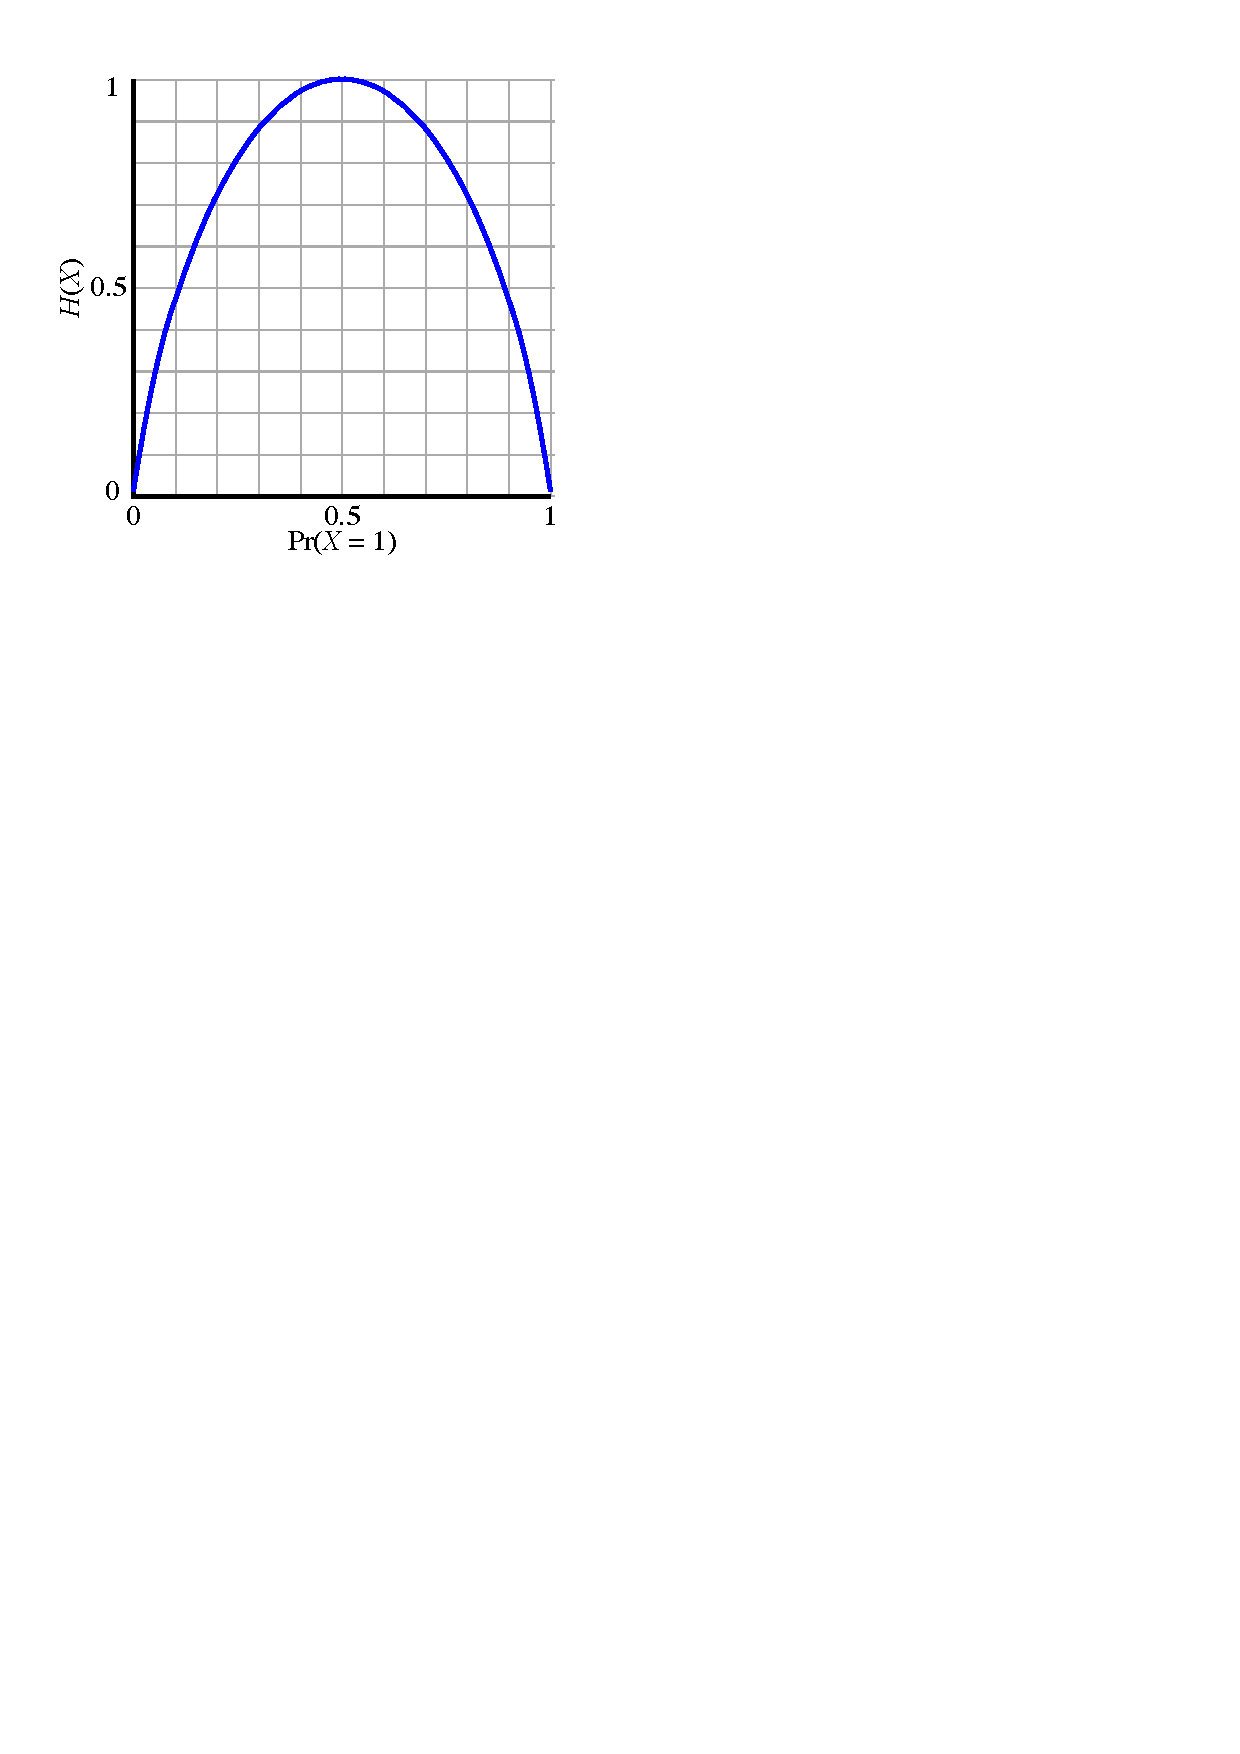
\includegraphics[width=1.3in]{figures/Binary_entropy_plot.pdf}
\end{center}
\end{minipage}

\underline{Canonical example:} \hfill \\  % TA lecture 1/7/2015. 
\begin{tabular}{ l | r }
  X & Y \\ \hline
  0 & 1 \\
  1 & 0 \\
  1 & 1 \\
\end{tabular}
\hfill \\
If you want to estimate entropy of X, you can use P(X=0).  \hfill \\
\begin{align*}
	H[X] &= -[\frac{1}{3} \log_2 \frac{1}{3} + \frac{2}{3} \log_2 \frac{2}{3}] \\
		& = \frac{1}{3} \log_2 3 + \frac{2}{3} \log_2 3 - \frac{2}{3} \log_2 2 \\
		&= \log_2 3 - \frac{2}{3} \approx 0.91
\end{align*}
This time H[X] = H[Y] because of symmetry.  \hfill \\

The discrete distribution with maximum entropy is the uniform distribution.  For K values of X, $H(X) = \log_2 K$ \hfill \\  % book pg 57
Conversely, the distribution with minimum entropy (which is zero) is any delta-function that puts all its mass on one state. Such a distribution has no uncertainty. 
\hfill \\

\subsection{Conditional Entropy}
If you don't know x:  (this is kind of an average).  \hfill \\
$H[Y \mid X=x] = -\sum\limits_y P(Y=y \mid X=x) \cdot \log_2 P(y \mid X=x)$   \hfill \\
 $H[Y \mid X=x] =  E[S(Y \mid X=x)]  $  \hfill \\
Note that we are summing over y because we are specifying x. \hfill \\
\hfill \\

For a particular value of X:  \hfill \\
$H[Y \mid X] = \sum\limits_x p(x) H[Y \mid X=x]$  \hfill \\
\hfill \\

Back to table above: 
\begin{align*}
	H[Y \mid X=0] &= ?  \\
	& \mbox{look only at X=0 in table.}  \\
	&= -[0 + 1 \log_2]  \\
\end{align*}
Now that you know X=0, entropy goes to 0.   \hfill \\  \hfill \\

$H[Y \mid X=1] = 1$: You know \textit{less} if you know X=1. \hfill \\ \hfill \\

Now use 
$H[Y \mid X] = \frac{1}{3}(0) + \frac{2}{3}(1) = 2/3$ \hfill \\
Given X, you know more.  Average our the more certain case and the less certain case.  \hfill \\  \hfill \\

Note:  $H[Y \mid X] \leq H[Y]$: knowing something can't make you know less. 

\subsection{Entropy and Information Gain}
\textbf{Information Gain} -  $IG(X) = H(Y) - H(Y \mid X)$ \hfill \\
Y is the node on top.  X are the nodes below.  He might have used lower case.  \hfill \\
\textbf{Class Example}: If $X_1$ is a node for a split, and you want to know the information gain for that node, you:
\begin{itemize}
	\item calculate entropy of the split.  Find Entropy of each branch of the split, and the fraction of points that were channeled to each split.  E.g. %http://courses.cs.washington.edu/courses/cse446/16wi/Slides/2_DecisionTrees_Part2.pdf
	\begin{align*}
		\{T, T, T, T, T, F\} & \rightarrow \{T, T, T, T\} \mbox{ (for } X_1=T), \{T, F\} \mbox{ (for } X_1=F) \\
				& \rightarrow P(X_1 = T) = 4/6, P(X_1=F) = 2/6 \\
				& \rightarrow H(X_1 = T) =  (1*\log_2 1 + 0*\log_2 0) = 0 \\
				& \rightarrow H(X_1 = F) =  \frac{2}{6} (\frac{1}{2} \log_2 \frac{1}{2} + \frac{1}{2} \log_2 \frac{1}{2})  \\
				& = 1 \mbox{ (uniform distribution)} \\
				H(Y|X_1)  =  - \frac{4}{6} & (1*\log_2 1 + 0*\log_2 0) - \frac{2}{6} (\frac{1}{2} \log_2 \frac{1}{2} + \frac{1}{2} \log_2 \frac{1}{2}) \\
							& = 2/6
	\end{align*}
	\item find the entropy of the unsplit data:  $\{T, T, T, T, T, F\} \rightarrow -(5/6) \log_2(5/6) - (1/6) \log_2(1/6) = 0.65$  % check w/ google: -(5/6)*log_2(5/6) - (1/6)*log_2(1/6) == 0.65. 
	\item subtract the weighted average of the split entropies from the original: $IG(X_1) = H(Y) - H(Y|X_1) = 0.65 - 0.33$
\end{itemize}


%\textbf{Conditional Information Gain}:    \hfill \\ %$H(y|x) = -\sum P(y|x) log_2$ 
  \hfill \\

\begin{itemize}
	\item Low uncertainty $\leftrightarrow$ Low entropy.
	\item Lowering entropy $\leftrightarrow$ More information gain. 
\end{itemize}


\subsection{Bits}
If you use log base 2 for entropy, the resulting units are called bits (short for binary digits). \hfill \\ % book pg 57
How many things can you encode in 15 bits? $2^{25}$.  \hfill \\  % 1/11/2015 Lecture


\subsection{Common notation}
\textbf{semicolon versus $|$ in probabilities}: \hfill \\
E.g. $P(X ; \theta)$ vs $P(X | \theta)$

$|$ is for random variables and $;$ is for parameters.  

Andrew Ng verbalizes the semicolon as "parameterized by."  
So $f(x ; \theta)$ would be spoken as "f of x parameterized by theta"
	






\section{Decison Trees}
\smallskip \hrule height 2pt \smallskip




Let's do this thing. 

\end{multicols*}
\end{document}
